\chapter{Degrees}
Rishnak asked Ajur whether he knew about graphs and trees in mathematics. Ajur jumped up and down and proclaimed that he knew all about graph theory. He continued that graphs are often used to represent relations of a set of objects. Smiling broadly, he stated that the famous mathematician, Euler, was the father of graph theory. He was eager to show off his knowledge and described the famous  K\"{o}nigsberg bridge problem. K\"{o}nigsberg (now Kaliningrad in modern day Russia) was on the banks of the Pregel River.  There were seven bridges crossing this river, connecting the two sides of the river with two islands. Using a stick, Ajur drew a graph of this in the dirt.
\begin{figure}
\begin{center}
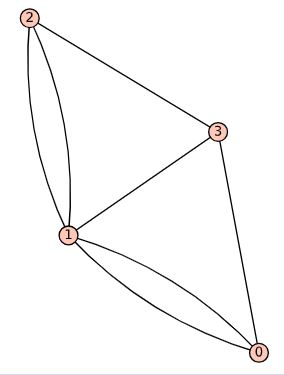
\includegraphics[width=0.6\textwidth]{konigsberg.JPG}
\caption{A graph representing K\"{o}nigsberg Bridge; vertices~1 and~3 are islands, whereas vertices~0 and~2 are the two riverbanks}\label{kon}
\end{center}
\end{figure}

He continued, stating that the problem was to start from the vertex labeled~0 and to walk across all bridges once and only once, finally returning to start vertex~0. Ajur could not contain his enthusiasm and asked Rishnak how to do it. Rishnak gently reminded Ajur that he was the one asking the questions and that Ajur had to respond with the correct responses. Ajur nodded his head.

Rishnak told Ajur, ``I am going to ask you a series of questions, then I'll observe whether I have any chance of having my curse lifted.''

Rishnak then asked Ajur, ``In a class of 33 students, what is the maximum and minimum number of friends a student can have? And since friend is a mutual relation, this means that if A is a friend of B, then B is a friend of A.  In other words, a student cannot be a friend to herself!''

Ajur replied nonchalantly that the maximum number of friends is~32 and the minimum number is zero.

Rishnak then asked Ajur, ``Will there be a student in the class with~32 friends and a student with zero friends?''

Ajur smiled to himself, seeing right away that Rishnak was a clever ghost.  Ajur replied, ``How is that possible?  If a student has 32 friends, she is friends with everyone else, so everyone else would have at least one friend.  So there cannot be a student with zero friends.''

Ajur paused and thought for a few seconds, then said, ``Similarly, if there is a student with zero friends, there are only~32 students remaining, so another student can have at most~31 friends.''

Rishnak was pleased to have found someone who seemed to have the ability to help him. His questioning continued.  ``Can all~33 students have a distinct number of friends? In other words, can each student have a distinct number of friends that differs from every other student?''

Ajur responded immediately by saying this was not possible because with~33 distinct students, the distinct number of friends each student in the class could have would be~$\{0,1,2,\cdots,32\}$. He smiled and said, ``And there are 33 numbers in this set, but alas, it contains both a students with~32 friends and a student with zero friends, which is not possible.''

Rishnak asked Ajur, ``Can there be just two students with the same number of friends, with the other students all having a distinct numbers of friends? And in this case, all of the students have at least one friend.''

Ajur frowned. This was not as easy a problem. There was no longer a student with zero friends. Ajur said, ``Give me a moment to reason this out.'' He knew that the maximum number could only be~32 and the minimum had to be one, otherwise there would not be~32 distinct numbers. But there are~33 students.

``Aha,'' said Ajur, ``by the pigeonhole principle, which states that if there are more pigeons than boxes, then one box must contain at least two pigeons, there has to be two students with the same number of friends.''

Rishnak said nothing, then asked, ``Are you sure that's it?''

Ajur quickly said, ``No, wait, there's more.''  He reasoned about what the numbers could be for each student. He matched~32 with one, i.e.,~the student with one friend has to be a friend of a student with~32 friends. Then he matched~31 with two, meaning the student with two friends has to be a friend of a student with~32 friends and a student with~31 friends. Continuing this argument, he matched~30 with three, 29 with four, $\cdots$, 18 with 15, and finally 17 with 16. He said, ``We have an even number of students accounted for, but an odd number of total students. So that means there are two students with the same number of friends.''

Rishnak moved on to the next question. ``If I asked five students in a class of six students how many friends each of them have and they all gave distinct numbers greater than zero, how many friends does the student who was not asked have?''

Ajur thought about this. ``Okay, if all five students had distinct numbers greater than zero, they had to be~$\{1,2,3,4,5\}$. Let's call the students A(pu), B(art), C(arla), D(uma), and E(rnie), with five, four, three, two, and one friend, respectively.''  As he spoke, Ajur drew a new diagram in the dirt. ``Let F(ermat) be the sixth student. A is friends with B, C, D, E, and F. B is friends with C, D, and F. B is already friends with A. And E has only one friend, namely A. Now C is friends with F. C is already friends with A and B. And D and E have their friends quota counted already. So it is easy to see from the graph that F has exactly three friends, namely A, B, and C.''

Ajur smiled and waved his hand majestically at the graph he drew [Figure~\ref{dg2}].

\begin{figure}
\begin{center}
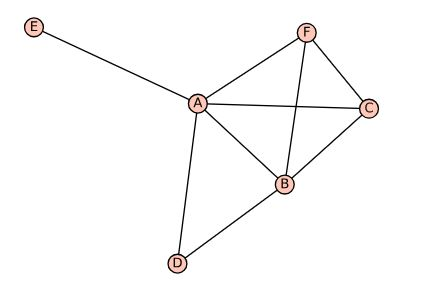
\includegraphics[width=0.6\textwidth]{graphstory1-1.JPG}
\caption{A graph with six students, with five students having 5, 4, 3, 2, and 1 friend}\label{dg2}
\end{center}
\end{figure}

Rishnak was impressed, but wanted to test Ajur even further. He asked whether there can be an odd number of students with a grand total of an odd number of friends. Ajur said that this was impossible as the sum of all numbers of friends across all students has to be even. He said, ``Look at it this way. If~A is a friend of~B, then this friendship is counted twice since~B is also a friend of~A. Hence the sum of all friends is even. We know that students with an even number of friends will contribute an even number of friendships (twice as many). And this in turn implies that the number of students with an odd number of friends also has to be even since doubling an odd number always gives you an even number.''

Rishnak smiled, then said, ``Good. Next, can you draw a graph of a class with five students having one, one, two, two, and two friends?''

Ajur knelt and whipped up the graph in the dirt [Figure~\ref{dg3}].

\begin{figure}
\begin{center}
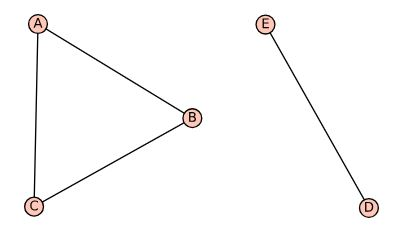
\includegraphics[width=0.5\textwidth]{graphstory1-2.JPG}
\caption{A graph with five students having 1, 1, 2, 2, and 2 friends}\label{dg3}
\end{center}
\end{figure}

Rishnak asked, ``Can you draw a different graph with the same number of friend relationships, meaning the same degree sequence?''\footnote{Hakimi has given a method of constructing a graph with a given degree sequence}

\begin{figure}
\begin{center}
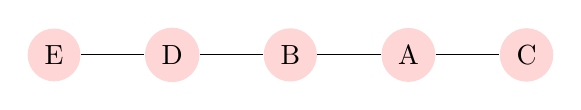
\begin{tikzpicture}
  [scale=.5,auto=left,every node/.style={circle,fill=red!16}]
  \node (n1) at (0,0) {E};
  \node (n2) at (3,0)  {D};
  \node (n3) at (6,0)  {B};
   \node (n4) at (9,0)  {A};
  \node (n5) at (12,0)  {C};
  \foreach \from/\to in { n1/n2,n2/n3,n3/n4,n4/n5}
    \draw (\from) -- (\to);

\end{tikzpicture} %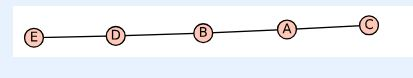
\includegraphics[width=0.6\textwidth]{graphstory1-3.JPG}
\caption{Another graph with five students having 1, 1, 2, 2, and 2 friends}\label{dg4}
\end{center}
\end{figure}

Ajur took no time to respond and drew another graph [Figure~\ref{dg4}].
Jura had long ago fallen asleep but now stirred. He barked, trying to tell Ajur that he wanted him to play. Rishnak was happy to hear the answers Ajur gave. He saw a ray of hope that his curse could maybe finally be lifted.

\subsection*{Question for the first day}
Rishnak stood tall in front of Ajur.  ``Okay, here is the question for the first night.  It has two parts.  Answer correctly and we'll continue again tomorrow. First, can you provide a degree sequence that is the degree sequence of exactly one graph? And ignore the labels on the vertices. They do not matter.''

Ajur started to answer, but Rishnak raised his hand, silencing him.  ``Wait, here is part two of the question. Is there also a degree sequence with exactly one graph that realizes it that has at least one edge?''

Ajur frowned.  ``Let me think.''

\textit{Before you turn the page, try to come up with answers of your own!}

\newpage
\subsection*{Answer for the first day}
Ajur said, ``For the first question, that's easy.  A degree sequence of all zeros can have only one graphical realization.''

Rishnak nodded. ``And to the second question? A degree sequence with exactly one graph that realizes it that has at least one edge?''

Ajur thought for a moment, then responded, ``Yes, for a sequence of even length, a degree sequence of all ones would always be realized by a unique graph.''
He used his stick to draw an example graph with a degree sequence of eight ones [Figure~\ref{daya1}].

\begin{figure}
\begin{center}
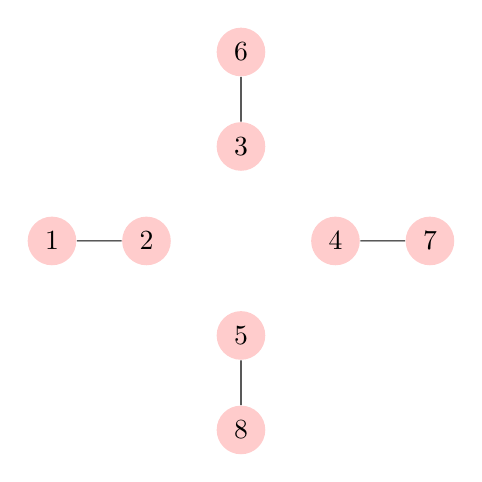
\begin{tikzpicture}
  [scale=.6,auto=left,every node/.style={circle,fill=red!20}]
  \node (n1) at (1,7) {1};
  \node (n2) at (3,7)  {2};
  \node (n4) at (7,7) {4};
  \node (n7) at (9,7)  {7};
  \node (n6) at (5,11)  {6};
   \node (n3) at (5,9) {3};
   \node (n5) at (5,5) {5};
   \node (n8)  at (5,3) {8};
  \foreach \from/\to in {n1/n2,n3/n6,n4/n7,n5/n8}
   \draw (\from) -- (\to);

\end{tikzpicture}
\caption{A unique graph with degree sequence $\{1,1,1,1,1,1,1,1\}$}\label{daya1}
\end{center}
\end{figure}

Rishnak told Ajur to come back the next night. Ajur stood agape as Rishnak disappeared into a cold mist.